\section{\textit{Punaharmaa ja kahdeksas matkustaja}}

\thispagestyle{empty}
\ThisCenterWallPaper{1.01}{assets/liljat00}

\begin{figure}[!h]
\centering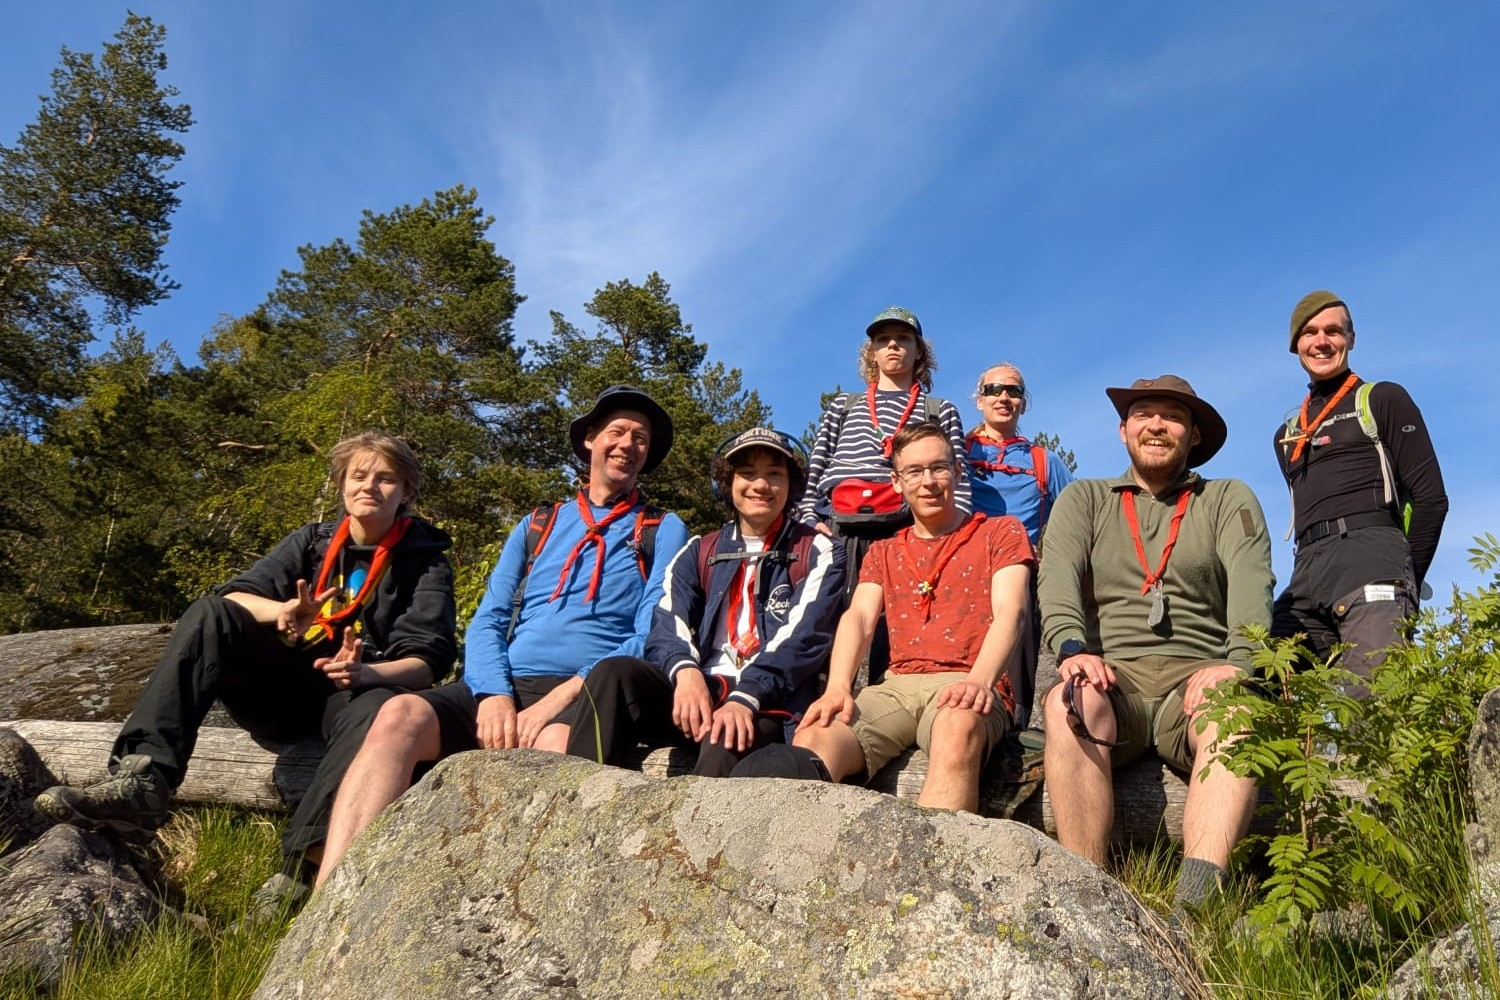
\includegraphics[width=\textwidth]{assets/liljaryhma.jpg}
\caption{\textit{Punaharmaa ja kahdeksas matkustaja} "=vartion ryhmäkuva 
Viikinrannan kalliolla, kun takana on jo yli 45 kilometriä.}
\end{figure}

\noindent\textit{Keväällä käveltiin punainen, viidenkymmenen kilometrin 
nahkalilja ja harmaa, kuudenkymmenen kilometrin nahkalilja. Liljaan kuuluu aina 
vartion kirjoittama raportti vaelluksesta. Raportti kirjoitetaan sekä vartiota 
itseään varten, jotta se voi pohtia ja mietiskellä yhteistä suoritustaan, 
että nahkaliljan myöntävää partiojohtajaa varten, jotta hän voi 
suorituksen tarkistaa; onhan se hauskaa palata ajassa taaksepäin ja lukea 
myöhemmin ajatuksista ja kommelluksista nahkaliljavaelluksilla! Tässä 
jutussa pääset lukemaan vartioiden yhdistelmäraportin.}

\begin{multicols}{2}
\begin{figure*}[!t]
\centering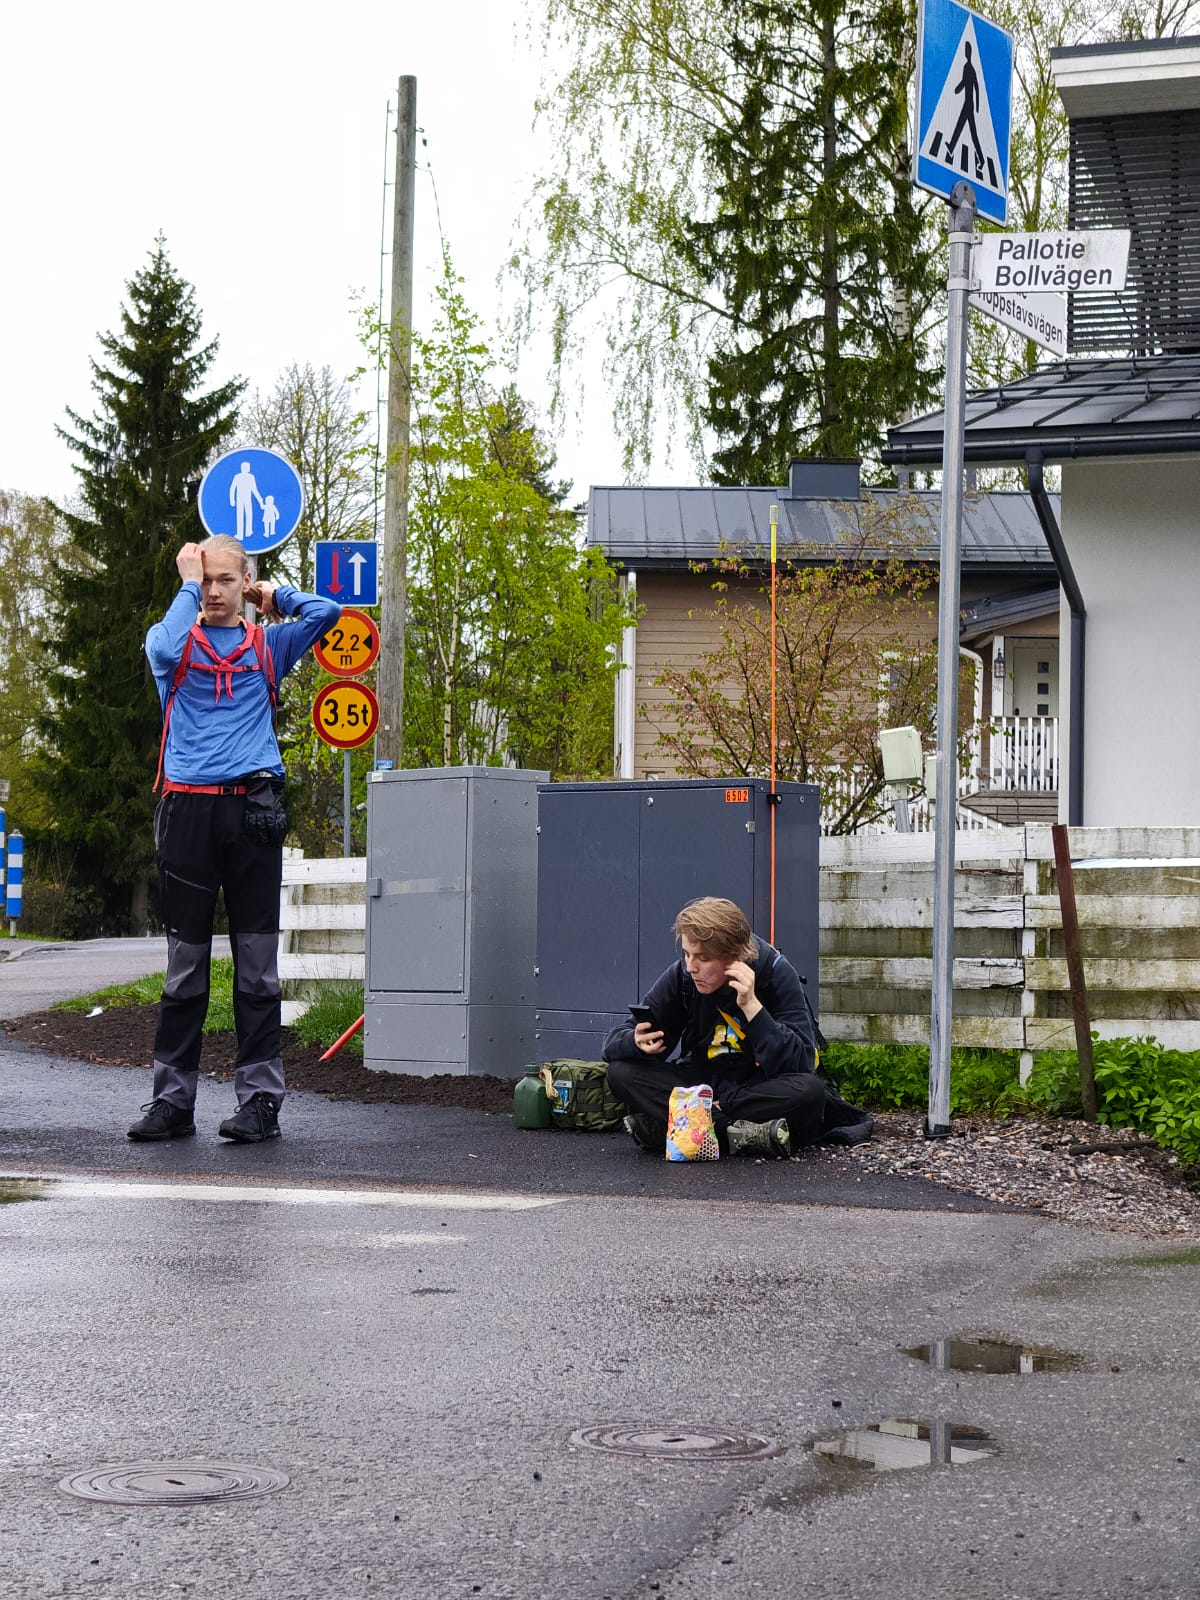
\includegraphics[width=.475\textwidth]{assets/nahkaliljaHarmaa1}\hfill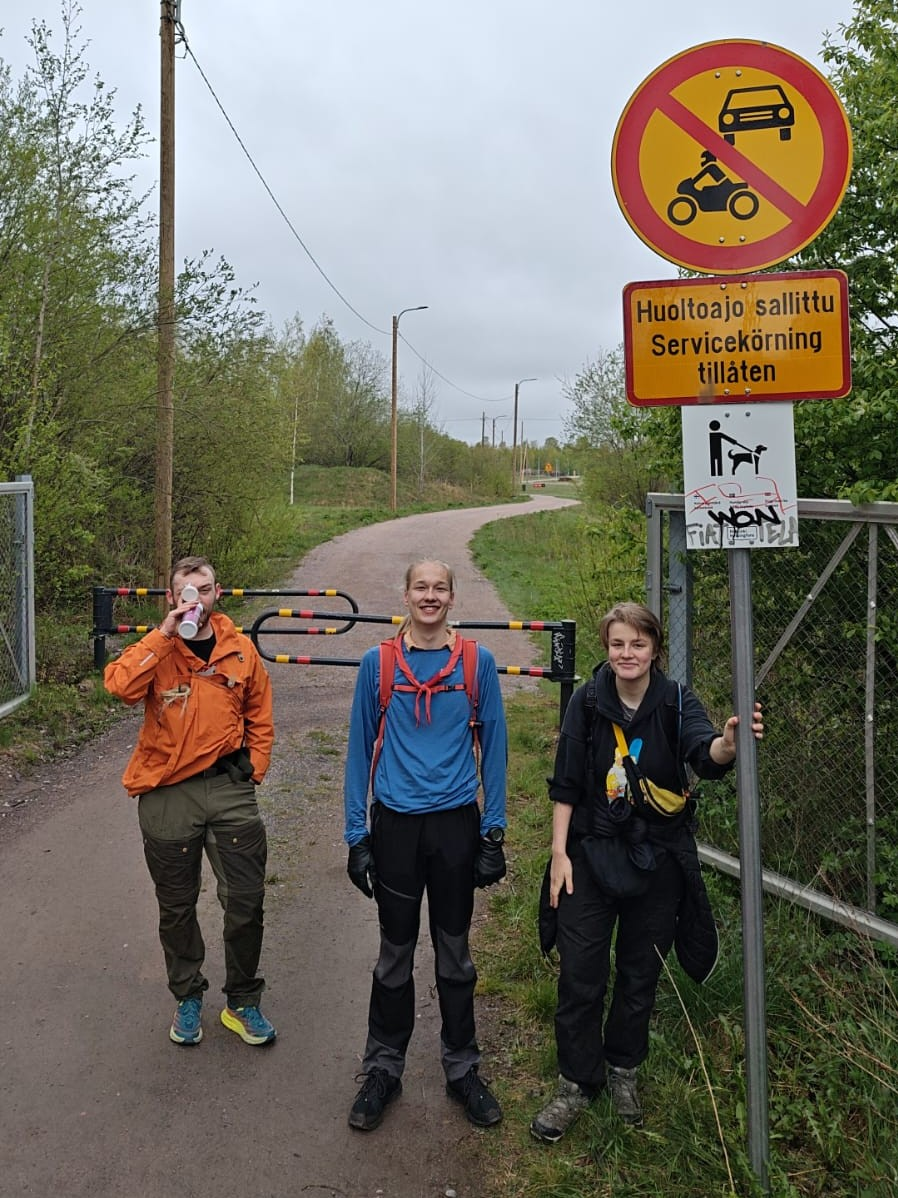
\includegraphics[width=.475\textwidth]{assets/nahkaliljaHarmaa2}
\caption{\textit{Harmaa}-vartio taukoilemassa nahkaliljan ensimmäisten 20 kilometrin aikana.}
\end{figure*}

\noindent Sateisena lauantain aamuna 17.5 neljä rusakkoa lähti Kontulasta Mikaelinkirkolta kello 6:03 ennakkoluulottomasti kävelemään harmaata nahkaliljaa. Nahkalilja on suoritus, jossa on 24 tunnin aikana käveltävä vaikeusasteen määräämä matka, harmaan liljan tapauksessa 60 kilometriä. Noin kymmenen minuutin kävelyn jälkeen sade lakkasi, mutta ilma oli kostea ja taivas pilvinen vielä jonkin aikaa. Kirkolta rusakot lähtivät kävelemään kohti Linnanpellon viljelypalstoja, mistä jatkettiin Mellunmäen läpi, missä viidennen kilometrin jälkeen pidettiin ensimmäinen tauko.

\thispagestyle{empty}
\ThisCenterWallPaper{1.01}{assets/liljat01}

Mellunmäestä matka jatkui kaakko-luode suunnassa Rajakylän läpi, kunnes saavuttiin Maratontielle, jota jatkettiin käytännössä sen koko pituus itään, kunnes käännyttiin Länsimäentielle pohjoiseen Kuusisillalle, missä kahden tunnin marssin jälkeen tuli vastaan Porvoonväylän yli menevä reitin ensimmäinen silta. Kuusisillalla tuli täyteen kymmenes kilometri, ja samalla sadas yhteinen kilometri nahkaliljoissa neljälle rusakolle. Kuusisillalta matka jatkui länteen Huoko- ja Suurmetsäntietä pitkin Jakomäen läpi kunnes Alppikylän jälkeen reitti alkoi kääntyä takaisin itään Tattarisuon ympäri, missä pidettiin kolmas tauko.

Tattarisuon jälkeen reitillä oli kolmas sekä neljäs silta sekä Lahden- että Porvoonväylän yli, kunnes matka jatkui Kivikkoon ja siitä takaisin kirkolle. Kirkolla pidettiin 20 kävellyn kilometrin kunniaksi hieman pidempi tauko, jolloin osa rusakoista kävi hakemassa kaupasta lisää evästä, yksi haki uudet kengät. Samalla mukaan otettiin myös punaista, eli 50 kilometrin pituista liljaa suorittava kolmen rusakon kokoinen osasto, sekä lippukunnanjohtaja, eli kahdeksas matkustaja, mikä huvitti 1980-luvun scifi-elokuvia katsoneita osallistujia.

{\smallskip\noindent\centering ***\par\smallskip}

Neljä rusakkoa, Alden, Elias, Janne ja Toivo, nahkaliljavartio 
\textit{Punainen ja neljäs matkustaja}, starttasi punaisen nahkaliljan, 
viidenkymmenen kilometrin vuorokausivaelluksen Mikaelinkirkolta suunnitellusti 
\textbf{kello 8.00}. Yön aikana oli satanut kolmisen milliä vettä ja tiet 
olivat märkiä, mutta sääennusteessa lauantaipäivästä povattiin varsin 
aurinkoista. Lähtöön saapui viimeisenä Toivo, joka saikin kunnian toimia 
kartanlukijana ensimmäisen viiden kilometrin etapin ajan.

Huolella suunniteltu kymmenen kilometrin kierros Kontulassa, Myllypurossa, 
Latokartanossa ja Kivikossa suuntasi ensin etelään kohti Kontulan 
kelkkapuistoa. Kävellessä keskusteltiin nahkaliljaan mukaan otetuista 
eväistä ja juotavista, kuinka aikaisemmista liljoista oltiin opittu ja nyt 
paremmin varauduttu. Öinen sade oli houkutellut etanat, kotilot ja lierot 
kävelyteille ja vartio olikin valmis uudelleennimeämään Hietajärvenpolun 
Etanapoluksi matkalla kohti Mustapuronpuistoa. (Toim. huom. tässä vaiheessa 
ei vielä tiedetty, että myöhemmin reitille osuisi oikea Etanapolku 
Yliskylässä.) Suurin osa kierroksesta oli hiekkatietä, minkä vuoksi 
erityisesti kotiloita jouduttiin väistelemään melkein koko aamu. 

Lähestyttäessä Myllypuroa vartion keskustelu oli rönsyillyt jo opettajiin 
ja heidän tunnetuksi tulleisiin lausahduksiin ja pian kavuttiinkin 
Alakivenpuiston kuntoportaita ylös entiselle jätemäelle ottamaan punaisen 
liljan suorittajista ryhmäkuva. Toivo seurasi reittiä ansiokkaasti, vaikka 
oikaisuvaihtoehto Myllytaipaleelle olikin houkutteleva: ''Hei, shortcut!''

Aikaisempien nahkaliljojen ja harjoitusmarssin muistelot siivittivät 
vaellusta. Ensimmäinen etappi oli taitettu \textbf{kello 9.03} ja vartio 
pysähtyi tauolle Hallainvuoren juurelle. Tauko päätettiin pitää lyhyenä, 
jotta ennätettäisiin takaisin kirkolle kymmeneksi. Kartta vaihtui Aldenille 
ja reitin suunta kääntyi pohjoiseen. Luonnonsuojelualueen reunalla mietittiin 
hauskoja paikannimiä -- mainittiinpa ainakin Ii, Yksipuinen ja Pöljä. 

Viikin puistosilta palautti mieleen kevään 2024 nahkaliljan, jossa osa 
suorittajista oli henkisesti romahtanut sillan päässä. Tällä kertaa silta 
ei tuottanut yhdellekään vartion jäsenelle ongelmia, askel oli kevyt ja 
Alden tokaisi: ''I'm feeling really happy.''

Paukkulanpuistoon saavuttaessa arvuuteltiin, josko vartio törmäisi 
aikaisemmin kävelemään lähteneisiin harmaan nahkaliljan suorittajiin, 
\textit{Harmaa}"-vartioon. \textit{Punainen ja neljäs matkustaja} osoittautui 
olevan kuitenkin yli kymmenen minuuttia \textit{Harmaata} edellä, joten 
pysähtymättä jatkettiin kohti Kivikon ulkoilupuistoa. Aivan sattumalta 
vartiota tervehti neljä rusakkoa lumilautailurinteelle vievässä 
ylämäessä. Ehkä nekin olivat lauantaikävelyllä!

Reitin kaartaessa takaisin kirkolle päin puheenaihe oli vaihtunut Hawkingin 
säteilyyn, jota Toivolla oli haasteita kuvailla. Säästämme lukijoilta 
säteilyn varsinaisen määritelmän, mutta kukin voi halutessaan sen verkosta 
tarkistaa. Juuri parahiksi aurinko alkoi pilkistää pilvien välistä vartion 
saapuessa kirkolle \textbf{kello 10.06}. Kirkolla pidettiin vajaan tunnin 
tauko, jonka jälkeen yhdistelmävartio \textit{Punaharmaa ja kahdeksas 
matkustaja} jatkoi matkaa yhteiselle neljänkymmenen kilometrin kierrokselle. 

{\smallskip\noindent\centering ***\par\smallskip}

Kirkolta matkaa jatkettiin itään Kontulan ja Mellunmäen läpi kohti Mustavuorta, missä pidettiin viides tauko kuusistossa. Siitä matka jatkui ylöspäin Vuosaaren huipuille, ensimmäisenä eteläiselle- ja sen jälkeen pohjoiselle huipulle, missä selkeytyneen sään takia maiseman ansiosta useampi tauko peräjälkeen niin, että kun Niinisaarentiellä pidettiin tauko, oltiin jo seitsemännessä. Siitä matka jatkui vartiokylän pohjoispäässä olevan reitin sillan yli, joka oli reitin neljäs. Vartiokylänlahden rantoja jatkettiin länsipuolella aurinkolaiturille asti, missä pidettiin seuraava astetta pidempi tauko kolmannenkymmenennen kilometrin merkiksi.

Siitä matka jatkui lounaaseen Puotilan läpi Strömsinlahden puistoon, missä pidettiin tauko, jonka jälkeen matka jatkui Tammisalon läpi Laajasaloon, jolloin saarten välillä hyppiessä ylitettiin sekä viides että kuudes silta. Laajasalon Alepan edustalla pidettiin seuraava tauko, jonka aikana osa rusakoista osti jäätelöä. Lähes heti tauon jälkeen Tullisaaressa täyteen tuli 40 käveltyä kilometriä. Matka Laajasalosta jatkui Herttoniemen läpi, missä matkaan mahtui reitin seitsemäs silta. Matkalla ohitettiin kahden liljan takainen puolimatkan krouvin pitopaikka, mutta tällä kertaa siinä ei taukoa jääty pitämään, vaan 11. tauko, joka oli ensimmäinen laatuaan noin kuuteen kilometriin, lykättiin Herttoniemen koiliskulmaan, hieman ennen Viikin Arboretumiin siirtymistä.

Pian tämän jälkeen saavuttiin Viikin arboretumiin, jonka rusakot halkaisivat kaakko-luode suunnassa, ja jonka loputtua täyteen tuli harmaan liljan kävelijöiden 50. kilometri, ja Viikintien varrella pidettiin rakonpaikkaustauko jolla käytettiin nyt jo lopussa olevaa urheiluteippirullaa, joka lähdössä oli ollut täysi. Viikintieltä matka jatkui pohjoiseen Vantaanjoen vartta pitkin Pukinmäkeen, missä ylitettiin yhdeksäs silta ensimmäisen kehätien yli, jota seurattiin itään Kivikkoon asti niin, että matkalle mahtui Pukinmäen S-marketin edustalle 14. tauko.

Kivikon Sortti-aseman jäädessä taakse osa suorittajista alkoi jäämään matkasta kotiinpaluun merkeissä. Ensin yksi punaisen liljan suorittaja jätti lippukunnanjohtajan kanssa muun joukon Kivikonlaidan ja Kivikontien liikenneympyrässä, jossa muut jatkoivat pohjoiseen, kävelivät he bussin 560 Kurkimäen pysäkille. Seuraavana toinen punaisen liljan suorittaja hyppäsi Kurkimäentien pysäkillä 57 bussiin, mistä muut jatkoivat maaliin. Mikaelinkirkolle käveli Kivikon läpi ja lippukunnan vanhan kolon ohi Keinulaudantiellä koko harmaan liljan suorittanut osasto, joka lopussa oli kävellyt yhdessä 150 kilometriä nahkaliljoissa, sekä yksi punaisen liljan suorittajista. Reitin viimeinen, eli kymmenes, silta oli Lahdenväylän ylitys Kivikon laitamilla, ja viimeinen, eli 15. tauko pidettiin Kivikon Sortti-aseman edustalla. Loppujenlopuksi kaikki osallistuneet kävelivät matkansa loppuun saakka, ja matkan varrella liljan tunnuskappaleeksi valikoitui TikTakin Mennään minne vaan.

{\smallskip\noindent\centering ***\par\smallskip}

Punaisen ja harmaan nahkaliljojen reittien pituuksiksi tuli tarkistusmittausten 
jälkeen 49,4 ja 59,5 kilometriä, mitkä tarkoittivat noin 3,6 ja 3,8 
kilometrin tuntivauhteja. Muut siirtymät ja taukoliikkumiset mukaan lukien 
kaikki suorittajat saavuttivat liljoissa vaaditut matkat. 

Ilmatieteen laitoksen Kumpulan havaintoasemalla merkittiin vaelluspäivän 
sääksi selkeästä pilviseen, lämpötila 7--14 astetta, lounastuulta, joka 
kääntyi itätuuleksi, 1--4 metriä sekunnissa ja ilmankosteus 53--98 
prosenttia -- mitä erinomaisin nahkaliljakeli!
\end{multicols}

\vfill

\noindent\null\hfill Kuvat: Tanguy\\
\noindent\null\hfill Teksti: Ahti ja Janne
